\chapter{Methodology}\label{ch:B}
\section{Planning}
We agreed on working with the Agile methodology. We love working with this way of approaching the project development, because it allows us to be flexible and don't be afraid of changes that we can face in the future. Furthermore, the Agile methodology has several advantages over traditional ways of developing a software. As, shown below: \cref{ch:Ref} \newline
\large \textbf {4 Values of Agile}\newline
Individuals and interactions over processes and tools.\\
Working software over comprehensive documentation.\\
Customer collaboration over contract negotiation.\\
Responding to change over following a plan.\\
\vspace{0.2cm}
\newline 1-scrum: define roles, choose an idea, plan sprints, prioritize our project.
\newline 2-scrum: creating a sketch of the site design model, finalizing the idea with improvements, general analysis of other educational platforms.
\newline 3-scrum: making adjustments to the functionality, its expansion. Make up the finished design. Setting up a site on servers, setting up a site domain, all actions with the site platform.
\newline 4-scrum coding: what potential users of the site will see, their interaction with the site.
\newline 5-scrum: how the code will be written, what features will be on the site and how it will be tested.
\newline 6-scrum: the site is being tested by members who were not involved in the development process.
\section{Collecting data}
Data affects on how the project, the project idea is built on. Collecting data is one of the hardest and time consuming processes of project modeling phase.  \\
The level of uniqueness relies heavily on data. We collected data related to academic issues using resources provided below:\\
• Surveys. We created a survey to collect questions that were of concern to school pupils.\\
• Expert suggestions. To come up with various ideas on how to improve, how to scale our platform.\\
• Interviews from Secondary School children. To determine notable issues in every day school life of children.\\
• Foreign websites. To consider pros/cons of existing online learning management platforms.\\
• National websites. To define outstanding problems in a country scale in the chosen sector.\\
• Domestic platforms. To define missing functionalities, inconveniences of Domestic learning management platforms.
\section{Results}
According to the data we collected, we've seen some outstanding problems in online school environment. Because the platform has two roles: pupil and teacher, we will specify problems in two branches.
(The results of survey are true for the time documentation was written, by the time it may vary)\\
\textbf{For pupils:}\\
to view assignments (40\% of respondents)\\
to work on the platform through phone (33.3\% of respondents)\\
old design(20\% of respondents)\\
uploading the work (60\% of respondents)\\
to view total grade for school quarter (16.7\% of respondents)\\
no opportunity to view the subject plan in advance.(66.7\% of respondents)\\
no visual overview of overall progress (66.7\% of respondents)\\
\textbf{For teachers:}\\
to check pupils' work for plagiarism.(almost 100\% of respondents)\\
to create a subject in the platform.(50\% of respondents\\
to be able to divide the class into two in every subject, since at schools classes are mostly taught in two groups.(50\% of respondents)\\
to leave comments on each students' work.(almost 100\% of respondents)\\

We want to highlight especially on the lack of opportunity to preview the topics of the subject, because as pointed out in the PRD 
(\cref{sec:PRD}), learners need to get clear instructions and expectations regarding subject/tasks in order to stay motivated for studies. So that school student knows he/she is on the right wave. 
As we've noticed, school children need a system of bonuses. \\
Moreover, in a platform where school children have been uploading their homeworks, there was a leak from the personality security perspective. \\
To conclude, these are the gaps in educational platforms that are in use at schools nowadays. 
\section{Tools and materials}
Anti-plagiarism checker is one of our main functions. It is an essential tool in the way of gaining education.\\
The realization of antiplagiarism checker function involves three steps: \cite{gunawan2018implementation}\\
\textbf{1.} Text-preprocessing.\\
\textbf{2.} Keywords weighting.\\
\textbf{3.} Text relevance calculation\\ 
\subsection*{STEP 1. Document pre-processing steps}
Any document needs to be cleaned up from unnecessary commas, words before being processed for a certain purpose. Thus, there are some simple steps towards document checking process begins:\\
* Tokenization: where a document is treated as a string (or \hyperlink{thebag}{Bag of words}), and then partitioned into a list of tokens.\\
* Removing \hyperlink{stopwords}{stop words}: This step eliminates them.
To realize this, examining various methods\cite{ramos2003using, trstenjak2014knn, 9194665}, we made a choice on Term Frequency Inverse Document Frequency (TF-IDF) method. Because, it is easy to compute and it is cheap in calculation. 
\subsection*{STEP 2. TERM FREQUENCY - INVERSE DOCUMENT FREQUENCY}
The \hyperlink{tfidf}{TF-IDF} is a text statistical-based technique which has been widely used in many search engines and information retrieval systems. TF is used to measure that how many times a term is present in a document. Whether IDF assigns weights to the words. The inverse document frequency assigns lower weight to frequent words and assigns greater weight for the words that are infrequent. \cite{qaiser2018text} \\
TF-IDF can be considered as space efficient, because the length of TF-IDF vectors is equal to the size of the vocabulary. Thus, it is more than feasible for checking school assignments.\ref{ch:Ref} \\
Secondly, it is not a linguistically motivated tool and and the approach is inherently language independent, which allows to check the work written in any language.\cite{van2010automatic}\\
\subsubsection{TF-IDF Vectorizer method}
After data preparation step, we move on to the TfIdfVectorizer() method from the sklearn python library. This method computes the word counts, IDF values, and Tf-idf scores all using the same dataset. In other words, it considers overall document weightage of a word.  TfidfVectorizer weights the word counts by a measure of how often they appear in the documents. As a result, it converts text into a vector format.
\begin{center}
    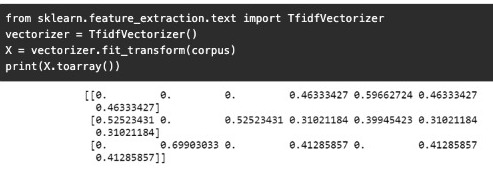
\includegraphics{vector.jpeg}
\end{center}
In the example above, text is added into the method and as a result we get vector, where its values are scores calculated for each word in the text.
\subsection*{STEP 3. Measuring similarity between two documents: }
After getting all the words converted into vector format, we apply similarity measurement method: $cosine_similarity$. Capturing the similarity of two documents using cosine similarity measurement. The cosine similarity is calculated by measuring the cosine of the angle between two document vectors. Using the formula: 
\begin{center}
    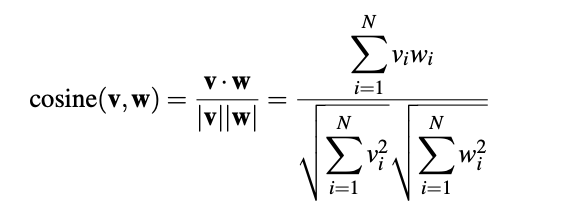
\includegraphics{formula.png}
\end{center}
\subsubsection{Cosine Similarity Measure}
The concept of similarity is fundamentally important in almost every field. Similarity is a core element in achieving an understanding of variables that motivate behavior and mediate affect. 
Cosine similarity is a measure of similarity between two vectors of n dimensions by finding the cosine of the angle between them, often used to compare documents in text mining. Given two vectors of attributes, A and B, the cosine similarity, is represented using a dot product and magnitude
as for text matching, the attribute vectors A and B are usually the tf vectors of the documents. The cosine similarity can be seen as a method of normalizing document length during comparison.
In \hyperlink{thisimage}{this image} it is illustrated how we applied the method in our implementation.\\
In the case of text retrieval, the result of cosine similarity will be between 0 and 1. If the result is closer to 1 (one), then it means the second document is significantly matching with the  reference
document.

